\section{Methodology}
\subsection{Finite Difference Method}
Finite Difference Methods(FDM) are used for approximating the solution of partial differential equations over a set of finite points, arranged in a geometrical structure called a \textbf{mesh}%
\footnote[1]{An object which consists of points which are spaced in a specific geometrical pattern is referred to as a \textbf{mesh} and each point in this mesh is called a \textbf{node}. The distance between any two adjacent nodes in a mesh with uniform spacing is called its \textbf{meshsize}}%
, in the continous domain of solution. The methods involve the idea of reducing the given PDE, by means of truncated taylor series approximation of the derivatives, to a difference equation which is much easier to digest numerically. 
\subsubsection{Finite Difference Approximations}
The quality of the solution depends on the quality of approximations made to the derivatives.
%%%
Consider this one-dimensional structured mesh of nodes $(x_0,x_1,x_2,..,x_i,..,x_n)$ at which the solution $U(x_i)$  is to be found, such that the difference $h = x_{i+1} - x_i $ is constant throughout the mesh and $x_i \equiv x_0 + ih$.\\
\begin{figure}[h]
\centering

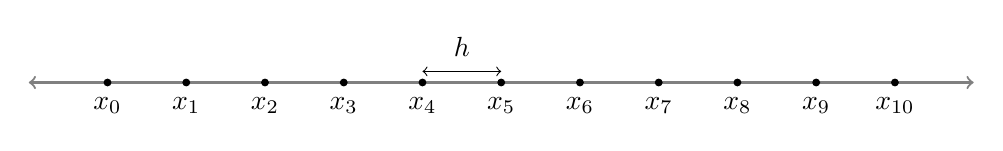
\begin{tikzpicture}
    \coordinate (H) at (4.5,6pt);
    \draw[thick,color=gray,<->] (-1,0) -- (11,0);
    \foreach \x  in {0,1,2,3,4,5,6,7,8,9,10}
        \draw[fill=black] (\x cm,0) circle (1.2pt) (\x cm,-2pt) node[anchor=north] {$x_{\x}$};
    \draw[thin,<->] (4,4pt) -- (5,4pt);%
    \node[anchor=south] at (H) {$h$};
\end{tikzpicture}

\caption{\small 1D mesh with 11 nodes and a meshsize h}
\end{figure}
\\
Let $U_i$ represent the solution at the $i$-th node and \hfill
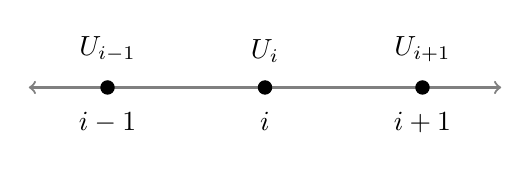
\begin{tikzpicture}[scale =2]
    \draw[thick,color=gray,<->] (3,-2cm) -- (6,-2cm);
    \foreach \x  in {3.5,4.5,5.5}
        \draw[fill=black] (\x cm,-2cm) circle (1.2pt) ;
    \draw (3.5 cm,-2.01cm) node[anchor=north,shift={(0,-5pt)}] {$i-1$};
    \draw (4.5 cm,-2.01cm) node[anchor=north,shift={(0,-5pt)}] {$i$};
    \draw (5.5 cm,-2.01cm) node[anchor=north,shift={(0,-5pt)}] {$i+1$};
    \draw (3.5 cm,-1.99cm) node[anchor=south,shift={(0,5pt)}] {$U_{i-1}$};
    \draw (4.5 cm,-1.99cm) node[anchor=south,shift={(0,5pt)}] {$U_{i}$};
    \draw (5.5 cm,-1.99cm) node[anchor=south,shift={(0,5pt)}] {$U_{i+1}$};
\end{tikzpicture}
\begin{equation*}
    \left. \frac{\partial U}{\partial x} \right|_{x_ i} = U_{x}(x_0 + ih) \equiv U_{x}|_i
\end{equation*} 
\begin{equation*}
    \left. \frac{\partial^2 U}{\partial x^2} \right|_{x_ i} = U_{xx}(x_0 + ih) \equiv U_{xx}|_i
\end{equation*}

The first order derivative can be defined as,
{\raggedright 
\begin{align*}
    &\text{} \hspace{1cm} U_x|_i = \lim_{h \to 0} \frac{U_{i+1} - U_i}{h}  \\
    &\text{or,} \hspace{1cm} U_x|_i = \lim_{h \to 0} \frac{U_{i} - U_{i-1}}{h}  \\
    &\text{or,} \hspace{1cm} U_x|_i = \lim_{h \to 0} \frac{U_{i+1} - U_{i-1}}{2h}  
\end{align*}
}

Finite difference approximations are obtained by dropping the limit and can be written as, 
 
\begin{flalign*}
    &\text{Forward Difference} \hspace{1cm} U_x|_i \approx \frac{U_{i+1} - U_i}{h} \equiv \delta^+_{x} U_i  \\
    &\text{Backward Difference} \hspace{1cm} U_x|_i \approx \frac{U_{i} - U_{i-1}}{h} \equiv \delta^-_{x} U_i \\
    &\text{Central Difference} \hspace{1cm} U_x|_i \approx \frac{U_{i+1} - U_{i-1}}{2h} \equiv \delta_{2x} U_i 
\end{flalign*}

Where $\delta^+_{x} , \delta^-_{x} , \delta_{2x}$ are called the \textbf{finite diference operators} for approximating \textbf{first-order derivatives} and their expansion is called the \textbf{finite difference quotient}, each representing forward,backward and centered respectively.
Second and Higher order finite difference Quotients can also be obtained,
\begin{align*}
    U_{xx}|_i &= \lim_{h \to 0} \frac{U_x(x_i+\frac{h}{2}) - U_x(x_i-\frac{h}{2})}{h} \\
    &= \lim_{h \to 0} \frac{1}{h} \left[{\frac{U(x+h) - U(x)}{h} - \frac{(U(x)- U(x-h))}{h}}\right]\\
    &= \lim_{h \to 0}\frac{U_{i+1}-2 U_i + U_{i-1}}{h^2} \\
    &\approx \boxed{\delta^2_x U_i \equiv \frac{1}{h^2}(U_{i+1}-2 U_i + U_{i-1})} \hspace{1cm} \text{[Central second-order Difference]}
\end{align*}

\begin{figure}[h]
    \centering
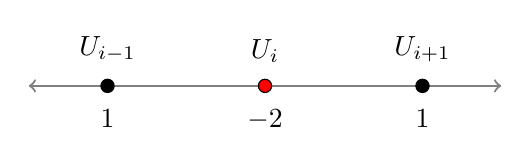
\begin{tikzpicture}[scale=2]
    \coordinate (A) at (3.5 cm,0cm);
    \coordinate (B) at (4.5 cm,0cm);
    \coordinate (C) at (5.5 cm,0cm);
    \draw[thick,color=gray,<->] (3cm,0) -- (6cm,0);
    \draw[fill=black] (A) circle (1.2pt) (A) node[anchor=north,shift={(0,-5pt)}] {$1$};
    \draw[fill=red] (B) circle (1.2pt) (B) node[anchor=north,shift={(0,-5pt)}] {$-2$};
    \draw[fill=black] (C) circle (1.2pt) (C) node[anchor=north,shift={(0,-5pt)}] {$1$};
    \draw (A) node[color=black,anchor=south,shift={(0,5pt)}] {$U_{i-1}$};
    \draw (B) node[color=black,anchor=south,shift={(0,5pt)}] {$U_{i}$};
    \draw (C) node[color=black,anchor=south,shift={(0,5pt)}] {$U_{i+1}$};
\end{tikzpicture}
\end{figure}

The vector of coefficients of the function values at various nodes forms what is called the \textbf{stencil} of the finite difference operator and it uniquely idetifies the operator. The combination $(1,-2,1)$ is called a \textbf{three point stencil} as it combines function values from three different points on the mesh.
It is fairly obvious to notice that any finite difference operator for any derivative at any node is just a linear combination of the function values at various neighbourhood nodes.   

\subsubsection{Local Truncation Error of Finite Difference Approximations}
The \textit{'error'} that accompanies \textit{'approximations'} in the method must be acccounted for. In this section, the truncation error in the derivative approximations is ascertained which will later help us deduce the error in PDE's solved using these approximations.
\\[2mm]
\textbf{The local truncation error for derivative approximations} is defined here as the difference between the exact value of the derivate and the approximated value at node $i$, it can be calculated using Taylor series expansions about $i$,\\[2mm]
For Forward difference operator, 
\begin{align*}
    \tau &\equiv \delta _ x^{+} U_ i - {U_ x}|_ i \\
    &= \frac{1}{\sDelta x}\left( U_ {i+1} - U_{i}\right) - {U_ x}|_i \\
    &= \frac{1}{\sDelta x}\left[ \left( U_ i + \sDelta x{U_ x}|_ i + \frac{1}{2}\sDelta x^2{U_{xx}}|_ i + \mcm{O}(\sDelta x^3)\right) - U_i \right] - {U_ x}|_ i \\
    &= \frac{1}{2}\sDelta x{U_{xx}}|_ i + \mcm{O}(\sDelta x^2) = \mcm{O}(\Delta x)
\end{align*}
For Backward difference operator, 
\begin{align*}
    \tau &\equiv \delta _ x^{-} U_ i - {U_ x}|_ i \\
    &= \frac{1}{\sDelta x}\left( U_ i - U_{i-1}\right) - {U_ x}|_i \\
    &= \frac{1}{\sDelta x}\left[ U_ i - \left( U_ i - \sDelta x{U_ x}|_ i + \frac{1}{2}\sDelta x^2{U_{xx}}|_ i + \mcm{O}(\sDelta x^3)\right)\right] - {U_ x}|_ i \\
    &= -\frac{1}{2}\sDelta x{U_{xx}}|_ i + \mcm{O}(\sDelta x^2) = \mcm{O}(\Delta x)  
\end{align*}
For Central difference operator,
\begin{align*}
    \tau &\equiv \delta _ {2x} U_ i - {U_ x}|_ i \\
    &= \frac{1}{{2 \sDelta } x}\left( U_ {i+1} - U_{i-1}\right) - {U_ x}|_i \\
    &= \frac{1}{2 \sDelta  x}\Bigg[ \left( U_ i + \sDelta x{U_ x}|_ i + \frac{1}{2}\sDelta x^2{U_{xx}}|_ i + \frac{1}{6}\sDelta x^3{U_{xxx}}|_ i + \frac{1}{12}\sDelta x^4{U_{xxxx}}|_ i + \mcm{O}(\sDelta x^5)\right) \\
    &\qquad - \left( U_ i - \sDelta x{U_ x}|_ i + \frac{1}{2}\sDelta x^2{U_{xx}}|_ i - \frac{1}{6}\sDelta x^3{U_{xxx}}|_ i + \frac{1}{12}\sDelta x^4{U_{xxxx}}|_ i +\mcm{O}(\sDelta x^5)\right)\Bigg] - {U_ x}|_ i \\
    &= -\frac{1}{6}\Delta x^2 U_{xxx_ i} + \mcm{O}(\Delta x^4) = \mcm{O}((\Delta x)^2)
\end{align*}
where in the above expressions we assume that the Higher order derivatives of $U$ at $i$ are well defined. For a fairly small $\Delta x$ (less than 1) we can confidently say that $\bo(\Delta x^2)$ is samller than $\bo(\Delta x)$%
\footnote{The definition of the "big $\bo$" notation says that if for given functions $f(x)$ and $g(x)$ for $x \in S$ where S is some subset of $\mathbf{R}$, there exists a positive constant A such that $|f(x)| \leq A|g(x)|$ $\forall$ $x \in S$, we say that $f(x)$ is the "big $\bo$" of $g(x)$ or that $f(x)$ is of order of $g(x)$, mathematically given by $f(x) = \bo(g(x))$}%
. Thus we note that the centered difference approximation (second-order accurate) approximates the derivative more accurately than either of the \textit{one-sided diferences} which are first-order accurate.\footnote{Forward and Backward differences are also called one-sided differences}

Similarly, Approximation of second-order derivative,
\begin{align*}
    \tau &\equiv \delta^2_x U_i - U_{xx}|_i \\
     &= \frac{1}{(\sDelta x)^2}(U_{i+1}-2 U_i + U_{i-1})  - U_{xx}|_i \\
     &= \frac{1}{(\sDelta x)^2}\Bigg[ \left( U_ i + \sDelta x{U_ x}|_ i + \frac{1}{2}\sDelta x^2{U_{xx}}|_ i + \frac{1}{6}\sDelta x^3{U_{xxx}}|_ i + \frac{1}{12}\sDelta x^4{U_{xxxx}}|_ i + \mcm{O}((\sDelta x)^5)\right) - 2 U_i\\
    & + \left( U_ i - \sDelta x{U_ x}|_ i + \frac{1}{2}\sDelta x^2{U_{xx}}|_ i - \frac{1}{6}\sDelta x^3{U_{xxx}}|_ i + \frac{1}{12}\sDelta x^4{U_{xxxx}}|_ i +\mcm{O}((\sDelta x)^5)\right)\Bigg] - {U_ {xx}}|_ i \\
    &= \mcm{O}((\sDelta x)^2)
\end{align*}
Thus, the second-order derivative approximator is also second order accurate.

%%Second derivate %%
\subsubsection{Reducing PDE to a discretised difference equation}
First we decompose our continous domain $\Omega := [0,4] \times [0,4.4] $ of $U'(x,y)$ to a discretised one by overlaying it with a uniformly structured rectangular mesh of meshsize $\sDelta x=\sDelta y= h$ and working only on the nodes of the mesh. \\[2mm]
Number of nodes along x axis, $N_x = \frac{4}{h} + 1$  \\[2mm]
Number of nodes along y axis, $N_y = \frac{4.4}{h} + 1$  \\[2mm]

\begin{figure}
    \centering
    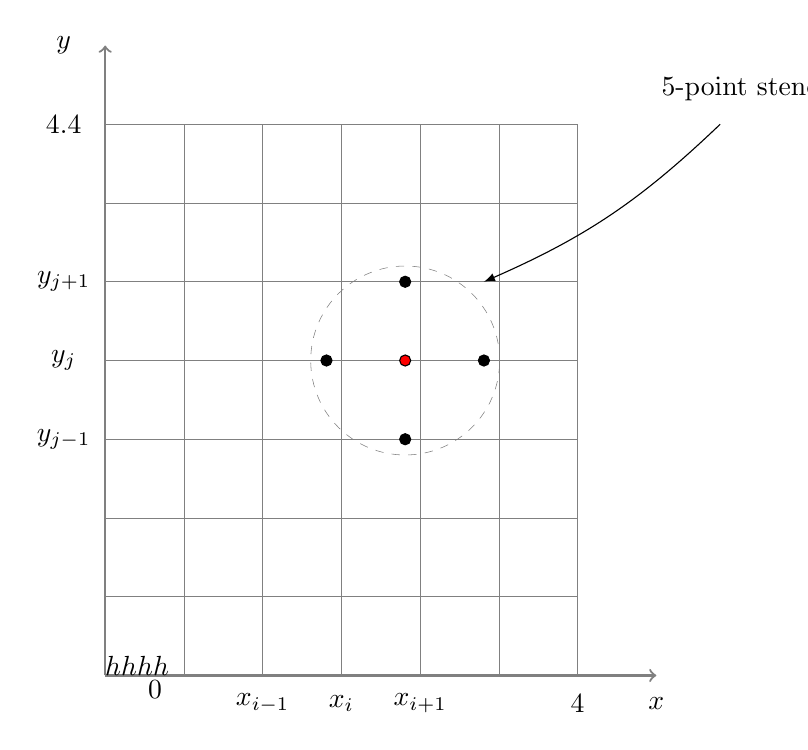
\begin{tikzpicture}
    \coordinate (Y) at (-15pt,8);
    \coordinate (X) at (7,-10pt);
    \draw[step = 1cm,gray, very thin] (0,0) grid (6,7);
    \draw[thick,color=gray,->] (0,0) -- (7,0);
    \draw[thick,color=gray,->] (0,0) -- (0,8);
    \draw (X) node {$x$};
    \draw (Y) node {$y$};
    \draw (X) node[shift={(-4,0)}] {$x_i$};
    \draw (Y) node[shift={(0,-4)}] {$y_j$};
    \draw (X) node[shift={(-5,0)}] {$x_{i-1}$};
    \draw (Y) node[shift={(0,-5)}] {$y_{j-1}$};
    \draw (X) node[shift={(-3,0)}] {$x_{i+1}$};
    \draw (Y) node[shift={(0,-3)}] {$y_{j+1}$};
    \draw (Y) node[shift={(0,-1)}] {$4.4$};
    \draw (X) node[shift={(-1,0)}] {$4$};
    \midlabelline{[shift={(-0.5,3cm + 10pt)}]X}{[shift={(-0.5,4cm +10pt)}]X}{$h$};
    \midlabelline{[shift={(-0.5,4cm +10pt)}]X}{[shift={(-0.5,5cm +10pt)}]X}{$h$};
    \coordinate (Xa) at ([shift={(2cm +15pt,-0.5)}]Y); 
    \coordinate (Xb) at ([shift={(3cm +15pt,-0.5)}]Y); 
    \coordinate (Xc) at ([shift={(4cm +15pt,-0.5)}]Y); 
    \midlabelline{Xa}{Xb}{$h$};
    \midlabelline{Xb}{Xc}{$h$};
    \draw (0,0) node[shift={(-5pt,-5pt)}] {$0$};
    \draw[fill=red] (3,4) circle (2pt) ;
    \draw[fill=black] (4,4) circle (2pt) ;
    \draw[fill=black] (2,4) circle (2pt) ;
    \draw[fill=black] (3,3) circle (2pt) ;
    \draw[fill=black] (3,5) circle (2pt) ;
    \draw[dashed,very thin,color=gray] (3,4) circle (1.2cm) ;
    \draw [latex-] (4cm,5cm) to [bend right=10] (7,7) node[anchor=south,shift={(10pt,5pt)}] {$5$-point stencil};
\end{tikzpicture}
\end{figure}
Therefore we have,
$U'_{i,j} = U'(x_i,y_j)$ and $\rho'_{i,j} = \rho'(x_i,y_j) \gs \forall \gs i \in 0,1,\dots,N_x -1 ; \gs j \in 0,1,\dots,N_y -1  $. \\[2mm]
We replace the second-order derivatives in partial differential equation (2.16) with central difference operators,
\begin{align}
    &\delta^2_x U'_{i,j} + \delta^2_y U'_{i,j} = - \frac{\rho'_{i,j} s^2}{\epsilon_0 \nu} \\
    &\frac{1}{h^2}(U_{i+1,j}+ U_{i-1,j} -4 U_{i,j} + U_{i,j+1}+ U_{i,j+1}) = - \frac{\rho'_{i,j} s^2}{\epsilon_0 \nu}
\end{align}

After rearranging we obtain the useful relation,
\begin{align}
    U_{i,j} = \frac{1}{4} \left[ U_{i+1,j}+ U_{i-1,j} + U_{i,j+1}+ U_{i,j+1} + h^2\frac{\rho'_{i,j} s^2}{\epsilon_0 \nu} \right]
\end{align}


\subsection{Iterative methods to solve linear algebraic equations}

In the last section we have discussed how to reduce a PDE to a linear combination of function values at various nodes by means of the method of finite differences. If we let the function value at any node as an unknown variable then the stencil when applied to all interior nodes gives rise to a system of linear algebraic equations, which may be very large. A two-dimensional problem like ours may lead to a system of several thousand unknowns, and three-dimensional problems involving several hundred thousand unknowns are common in real engineering situations. The solution of such a system is a major problem in itself as traditional methods like Gaussian-elimination result in large computation times, we are therefore forced to employ faster methods. As we have seen above, the system of equations produced by a discretisation has many special features and an efficient solution procedure must exploit these. The most obvious property of the system is that it is extremely sparse. Even when there are many thousand unknowns, each equation will involve one unknown and the unknowns at its immediate neighbourhood. In particular, if we write the equations in the conventional notation,
\begin{equation*}
    A \mvec{x} = \mvec{b} 
\end{equation*}
where A is an N × N matrix, b the given data vector and x the vector
of N unknown interior mesh values, there is an implied one-dimensional
ordering of these values which is somewhat unnatural and obscures the
important property that only immediate neighbours are involved. Each
row of the matrix A involves only a very small number of non-zero
elements, commonly five or seven; moreover in many problems a suitable
ordering of the unknowns will lead to a matrix in which these non-zero
elements occur in a regular pattern. In devising efficient methods for
the solution of the system these structural properties will be important,

\subsubsection{Jacobi Method}
\begin{algorithm}
	\caption{Jacobi Method}
	%{This iterative method takes an initial matrix of guess values and solves the the equation $$ Ax = b $$})
	\KwData{INPUT -: An $ k \times m $ matrix of initial values, value of step size $h$ and  also a matrix containing the initial charge configuration} 
	\KwResult{OUTPUT -: An $ k \times m $ matrix containing the values of potential on all $x$ and $y$ values} 
	\For{f = 0, 1, 2, 3, 4....N}{ 
		make new array of size $ k \times m $ \tcc*{initialising a new array for solution}
		\For(\tcc*{taking a x value}){i =0, 1, 2, 3 ... k}{
			\For(\tcc*{taking all y value for a x value}){ j =1, 2, 3 ... (m-1)}{
				\tcc{now defining the required quantites for stencil}
				$left = {a}_{i,j-1}$ \; 
				$right = {a}_{i,j+1}$ \;
				\If{$ i = k-1 $ }{
					$up = {a}_{i-1,j}$\;
					\Else{
						up = ${a}_{i+1,j}$\;
						
					}							
				}
				\If{ $ i = 0 $}{
					down = ${a}_{i+1,j}$\;
					\Else{
						down = ${a}_{i-1,j}$ \;
					}
				}
				{new ${a}_{i,j}$ = (up + down + left + right + $h^2 * {p}_{i,j} $ )/4 + new ${a}_{i,j}$} \tcc*{new value the grid point}
			}
			{max relative error = max(new  x - x)/ $x$}\;
			\If(\tcc*{checking for tolerance}){max relative error < tolerance}{
				{break}\;
				\Else(\tcc*{if tolerance not reached then the iteration continues}){
					new x =  x	
				}
			}
		}
	}	
\end{algorithm}
\subsubsection{Gauss-Seidel Method}
\subsubsection{Relaxation methods and Successive Over-Relaxation(SOR)}


